\documentclass[conference]{IEEEtran}
\IEEEoverridecommandlockouts
% The preceding line is only needed to identify funding in the first footnote. If that is unneeded, please comment it out.
\usepackage{cite}
\usepackage{amsmath,amssymb,amsfonts}
\usepackage{algorithmic}
\usepackage{graphicx}
\usepackage{textcomp}
\usepackage{xcolor}
\usepackage{anyfontsize}
\usepackage{hyperref}
\def\BibTeX{{\rm B\kern-.05em{\sc i\kern-.025em b}\kern-.08em
    T\kern-.1667em\lower.7ex\hbox{E}\kern-.125emX}}
\begin{document}

\title{TIII Cab Service\\
{\fontsize{15}{6}\selectfont Ruchitha Jujjuru}\\
{\fontsize{15}{6}\selectfont IIIT Hyderabad}\\
{\fontsize{15}{6}\selectfont jujjuru.ruchitha@students.iiit.ac.in}\\
}

\author{}

\maketitle





\section{Abstract}
At this paper, we will address the difficulties faced by students, instructors, and other staff members in the new extended institution in conducting tests, attending offline classes, and other tasks that require high timeliness by designing a cab service system as they are now residing in far away parts from each other.


\section{Introduction}
Everyone wants a massive campus like TIII, yet everything has advantages and disadvantages. As a result, there are some issues that various college residents are experiencing that need to be addressed. usually From dawn until evening, classes and tutorials are held. Because the hostels, mess halls, and academic block are so far apart, many students are having a difficult time getting to class on time, which is affecting their academic performance and attendance marks. It would be difficult for students to attend lessons or examination rooms if they were scheduled right after supper time and in such a short period of time. If students fail to get to the exam centre on time and perform poorly as a result of the lack of time, it may jeopardise their entire semester's hard work.\par
It is necessary to ensure that the great distance between buildings does not interfere with any student's academic life.
To address this, and to ensure that no student misses any tests, key meetings, or interviews, and to ensure that distance is no longer a problem that detracts from a student's campus life experience, a  cab service service is a must.\par


\section{Literature Review}
Cab service is not new to Bhagyanagar or other large cities. Every cab service uses a nearly identical system to book rides, pay drivers, and so on. While this may be the case in the outside world, where technologies such as Google Maps provide clear data on where roads are blocked, where traffic is heavy, and other such facts, this may not be the case in the inside world. Some of these things work differently inside private universities, where roadblocks may be in place at certain intersections and certain areas are restricted to a select few. While Google Maps can provide a route to the college, it cannot understand inner information such as this. \par
some of the cab services we know are:\\
\begin{itemize}
\item Uber Cab Sevices:\\
In 2008, the Uber concept was conceived in Paris. They've evolved into a worldwide platform that enables flexible incomes as well as the movement of people and things in ever-increasing ways. You've progressed from four-wheeled connecting rides to two-wheeled freight deliveries to 18-wheeled freight deliveries. From background checks for drivers to real-time verification Uber also offers cab services in Bhagyanagar.\\
You can visit the site : \href{https://www.uber.com/in/en/}{Uber(Click Me)}
\item Mega Cabs:\\
Mega Cabs is an Indian radio taxi service that operates in six cities and has a fleet of 2,500 vehicles. Kunal Lalani launched the company in 2002. It is one of the country's first radio taxi services.
In the places where it operates, it provides dedicated airport transports, as well as a premium airport transfer service in Delhi/NCR.
It also provides outstation services throughout India, as well as last-mile connectivity and personnel transportation. Cab reservations can be made via the website, the hotline, or the dedicated app, which is available on all mobile platforms.\par
You can visit the site : \href{https://www.megacabs.com/}{Mega(Click Me)}
\item ola cab services:\\
Ola is India's leading mobility platform and one of the world's top ride-hailing companies, with operations in more than 250 locations across India, Australia, New Zealand, and the United Kingdom. The Ola app connects clients to drivers and a variety of vehicles, including motorcycles, auto-rickshaws, metered taxis, and cabs, allowing hundreds of millions of customers and over 1.5 million driver-partners to enjoy convenience and transparency. Bhavish Aggarwal and Ankit Bhati established Ola in December 2010 with the goal of providing transportation to a billion people.\par
You can visit the site : \href{https://olacabs.com/}{Ola(Click Me)}
\end{itemize}









\section{System Architecture}
As it goes by with all the cab booking companies I would also like to create an app to allow the users to book rides. Since almost everyone in the college would have their own digital devices either laptops or smartphones with internet connection, I have designed this app such that it can be accessed using any smartphone or laptop.

\subsection{Users}
\begin{itemize}
\item customer: it includes students,faculty,staff and other workers belonging to the  college.
\item Employee: it includes the employees/operators who are managing the cab services system in the college.
\item Driver: it includes the drivers who are employed by the college to drive the cabs. 
\end{itemize}
\begin{figure}[htbp]
\centerline{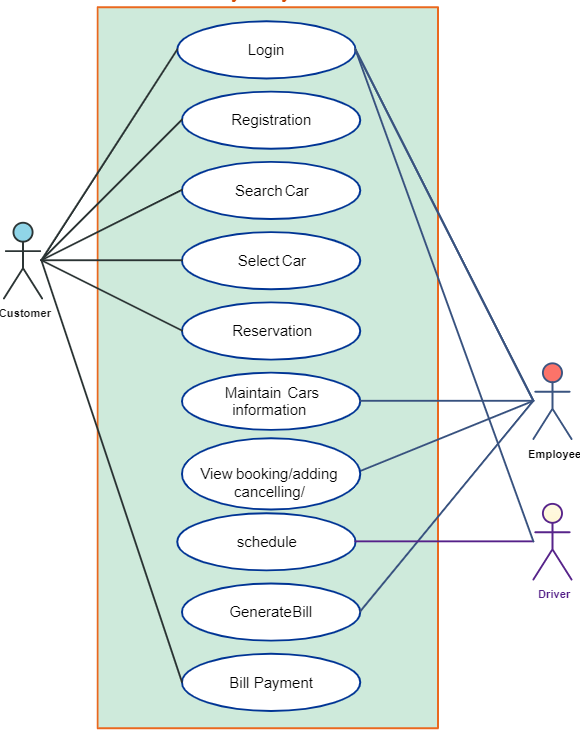
\includegraphics[scale=0.75]{usecase.png}}
\caption{UML Use case diagram}
\label{fig}
\end{figure}

\subsection{Main workflow}
\begin{itemize}
\item user makes an account in the web app of cab services with the institute mail id.And his details are added to the cab services database.

\item whenever the user wants to access the services , He /she login with the institute id .
\item each of the drivers are associated one of the cabs.
\item The user search for the available cars and selects one of them to reach his desired destination.
\item The employee vie the booking ,  generate bill , and the user pays the bill and reserve the car.
\item The employee then schedule the the respective car to the corresponding user.
\item If the user cancels the booking , the amount paid for the ride will be refunded.
\item Employee maintains the cab services database by updating and modifying information.
\end{itemize}

\subsection{Features}
\begin{itemize}
\item Login : User logins with institute email id .
\item Registration : New user has to register using institute email id providing other personal details.
\item Search Car : User can search for the available cab rides.
\item Select Car : User can choose the type of car from available rides.
\item Reservation : Confirm booking after bill payment.
\item Bill payment : Paying Bill for booking rides.
\end{itemize}

\subsection{Requirements}
The various requirements can be drawn in use case diagram (Fig1).
\begin{itemize}
\item User management: A safe and secure method to create accounts and authorize logins. There should also be a way to check the  database to ensure that the data provided is correct.
\item Rating System: A rating system for each ride should be implemented to analyse how helpful the service is. Services can be improved depending on the feedback of users.
\item Ride History : Ride History of each user would be maintained separately in order to recommend rides in future and also to provide coupons analysing the previous rides.

\end{itemize}
\subsection{ Classes used}
The different classes used are as described in 
\href{https://iiitaphyd-my.sharepoint.com/:f:/g/personal/jujjuru_ruchitha_students_iiit_ac_in/Evyw5AfMy19JpH4KClBtnaIBoQvmyfHD7ZdB8GWuyUEfBg?e=yMrs6y}{class diagram(Click Me)}
\begin{itemize}
\item User: this represents a user with email id and password. A user can specialize into an employee or driver or a customer .
\item employee: This represents the  employee who
is responsible for adding or cancelling booking ,maintaining cars information in database.
\item customer: This represents resident  of the
college who has access to the cab services.
\item driver: This represents driver employed to drive the cars.
\item college database: This contains the
email id  of all the residents of the college. This is used for verifying the details provided by
the user.
\item cab services database:This contains the
details  of all the users registered including their booking history.

\end{itemize}
\subsection{some sequence diagrams}
\begin{itemize}
\item \href{https://iiitaphyd-my.sharepoint.com/:f:/g/personal/jujjuru_ruchitha_students_iiit_ac_in/Evyw5AfMy19JpH4KClBtnaIBoQvmyfHD7ZdB8GWuyUEfBg?e=yMrs6y}{Click me to view the sequence diagram for verification and registration of User
}
\item \href{https://iiitaphyd-my.sharepoint.com/:f:/g/personal/jujjuru_ruchitha_students_iiit_ac_in/Evyw5AfMy19JpH4KClBtnaIBoQvmyfHD7ZdB8GWuyUEfBg?e=yMrs6y}{Click me to view the sequence diagram for session authentication of User
}
\end{itemize}



\section{Conclusion and Future Work}
We can clearly see how the college dedicated cab system will help students and faculty to reach the required destinations in time. This will also provide job oppurtunity to many taxi drivers in the city. Now we can ensure that no student misses out any of his/her exams and classes\\
In future release:\\
1. I would like to add sharing cab option to students which will reduce the taxi demand load and also the fare for students\\
2. I would like to extend cab services to outside of college too just in case any student wants to go outside of college\\
3. I would like to add the trip booking service. Student groups can book cabs in advance to go on a trip\\


\section{References}
\begin{itemize}
\item \url{https://blog.grabon.in/top-5-best-cab-services-in-hyderabad-and-bangalore/}
\item \url{https://jugnoo.io/how-does-a-taxi-booking-app-development-work/#:~:text=After%20verifying%20the%20estimated%20fare,and%20the%20chosen%20payment%20option}
\item \url{https://www.bytestechnolab.com/blog/how-to-build-a-taxi-booking-app-a-complete-guide/}
\item \url{https://www.unicotaxi.com/blog/post/step-by-step-guide-taxi-booking-app-development}
\item \url{https://www.megacabs.com/}
\end{itemize}

\end{document}